%
% File acl2020.tex
%
%% Based on the style files for ACL 2020, which were
%% Based on the style files for ACL 2018, NAACL 2018/19, which were
%% Based on the style files for ACL-2015, with some improvements
%%  taken from the NAACL-2016 style
%% Based on the style files for ACL-2014, which were, in turn,
%% based on ACL-2013, ACL-2012, ACL-2011, ACL-2010, ACL-IJCNLP-2009,
%% EACL-2009, IJCNLP-2008...
%% Based on the style files for EACL 2006 by 
%%e.agirre@ehu.es or Sergi.Balari@uab.es
%% and that of ACL 08 by Joakim Nivre and Noah Smith

\documentclass[11pt,a4paper]{article}
\usepackage[hyperref]{acl2020}
\usepackage{booktabs}
\usepackage{graphicx}
\usepackage{times}
\usepackage{latexsym}
\renewcommand{\UrlFont}{\ttfamily\small}

\usepackage{microtype}

\aclfinalcopy % Uncomment this line for the final submission


\newcommand\BibTeX{B\textsc{ib}\TeX}

\title{Abstractive Text Summarization with Bidirectional LSTM - CNN/DailyMail}

\author{Justin Haysbert}\\
  Tulane University / New Orleans, LA \\
  \texttt{jhaysbert@tulane.edu} 
\date{}

\begin{document}
\maketitle
\begin{abstract}
	One of the main uses of LLM’s such as ChatGPT and Deepseek is for the  summarization of long complex articles. Text summarizers can save casual readers valuable time and energy and even offer up ideas for users wishing to summarize text themselves. I'm aiming to create a text summarizer capable of paraphrasing news articles from the CNN/DailyMail summarization dataset. My project utilizes abstractive summarization using both an LSTM with attention and the BART Model then compares their performances. This study should gauge how big the performance gaps are between transformers and classic neural net approaches. 
\end{abstract}


\section{Introduction}




With the development of LLM’s such as chatGPT and Deepseek text summarization has become the norm for those looking to digest large amounts of information quickly. Many make the choice to toss the article into chatGPT for summarization rather than spending hours reading. The performance of these LLM’s come from years of development and innovations. The transformer model has particularly had a huge impact on NLP and text summarization. My project aims to take things back to the times before transformers to test out LSTM models for summarization. This project details the performance of the BART transformer model and an Bi-LSTM with attention on the abstract summarization of the CNN/Dailymail news dataset. 



\section{Methods}

In my implementation I began preparing the CNN/DailyMail data by importing from kaggle and utilizing pandas dataframes. The raw dataset contained 287,113 training points but due to computational limitations I decided to train my model on only 40,000. This dataset was transformed by splitting the articles and highlights on whitespace and mapping tokens to indexes in a vocabulary. To build vocabulary, token frequency was counted from the training set keeping tokens that showed up at least twice. Plus four special source tokens and three extra target tokens were added. A collate function then pads each batch of sequences so that every batch matches in shape. 
My model is an encoder-decoder with attention. The encoder is a bidirectional LSTM that reads articles forward and backwards, producing context rich representations. The decoder is a unidirectional LSTM that at each step computes attention weights over encoder output, forms a context vector, then combines context with the previous word for a next word prediction. I initialize the decoder hidden state by linearly projecting the encoder's final forward and backwards states. During training I use teacher forcing 50 percent of the time feeding in the true prev token, or feeding in the models own prediction. 
Then for each word in the target summary the decoder attends over the encoder outputs to pull in context. This produces next word probabilities, repeating until and end of sew token is emitted. I train my model for three epochs with a batch size of 8 using the adamW optimizer at a LR=0.005 and a cross entropy loss that ignores padding.


\section{Results}

After training the Bi-LSTM model I got a training loss of 6.5 and a validation loss of 7.0. Upon testing my model it was unable to produce viable summarizations of the news articles, outputting random characters or illegible text. For example a summary of an article involving a crime againt young women resulted in the summary “police say found guilty to old year old year old year old was in the . . . . . . . . . . . . . . . . . . . . . . . . . . . . . . . . . . .”. This shows that the model was unable to learn meaningful patterns in the data. This likely occurred because the model was not trained for long enough due to the lack of computational resources. Due to model failure I decided to skip the ROUGE evaluation knowing that it would be a waste to compare against the transformer model. To substitute this test I decided to implement the pretrained BART and compare its output to my LSTM. The BART model was loaded in from hugging face and the dataset was tokenized using the BART tokenizer. The BART model unsurprisingly performed perfectly on the news articles outputting accurate summarization of the articles.

\begin{table}[ht]
\centering
% note that we can refer to tables generated by our Experiments.ipynb notbook.
\input{../notebooks/table.tex}
\caption{\label{tab:a_table} A caption. }
\end{table}

Figure~\ref{fig:a_label} shows a figure

\begin{figure}[ht]
	\centering
	% note that we can refer to figures generated by our Experiments.ipynb notbook.
	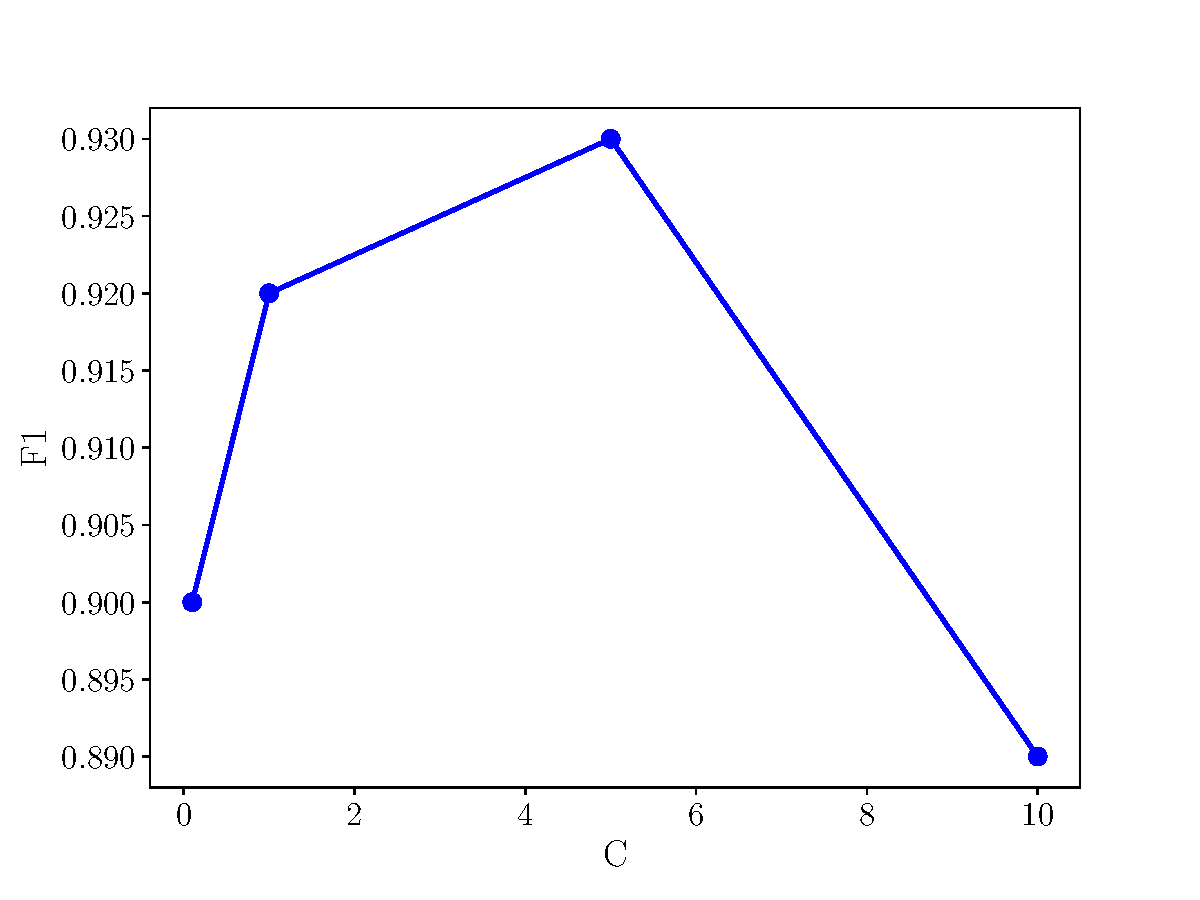
\includegraphics[width=3.5in]{../notebooks/results.pdf}
	\caption{A caption}
	\label{fig:a_label}
\end{figure}

\section{Discussion}

I initially used a Bi-directional LSTM for summarizing the CNN/DailyMail dataset, but it failed to produce coherent results. While the architecture was well-structured, the model wasn’t trained long enough or on a large enough subset of the data due to limited computational resources. As a result, the output was mostly gibberish. In contrast, the BART model performed exceptionally well on the same dataset—which isn’t surprising, given that it’s pretrained on 160GB of text. This highlights how transformer-based models, when paired with substantial data and compute, are highly effective for generating high-quality abstractive summaries.

\section{Conclusion}
This project demonstrated the challenge of training BI-Directional LSTM models for abstractive summarization on large datasets such as CNN/DailyMail, particularly under limited computational resources. Despite a solid architecture the LSTM approach failed to generate meaningful summaries due to insufficient training time and data exposure. In contrast the pre-trained BART model showed impressive results. This reinforces the value of transformer models with large scale data and computational resources. These results showcase that when attempting projects or specific NLP tasks it may be more time efficient to choose pretrained models. This project has allowed me the opportunity to explore the creation of text summarization and has allowed me to create a Bi-directional LSTM from scratch. It also gave me the opportunity to learn more about attention and its implementation in NLP tasks. 


\section{Division of Labor}
Justin Haysbert is responsible for all work presented in this project





\bibliography{references}
\bibliographystyle{acl_natbib}


\end{document}
